\section{Klassenhierarchie}
\label{sec:klassen}
Der Zugriff auf die in der bislang beschriebenen Datenbank gespeicherten Daten erfolgt über die folgende  Klassenhierarchie:

\begin{figure}[H]
\begin{center}
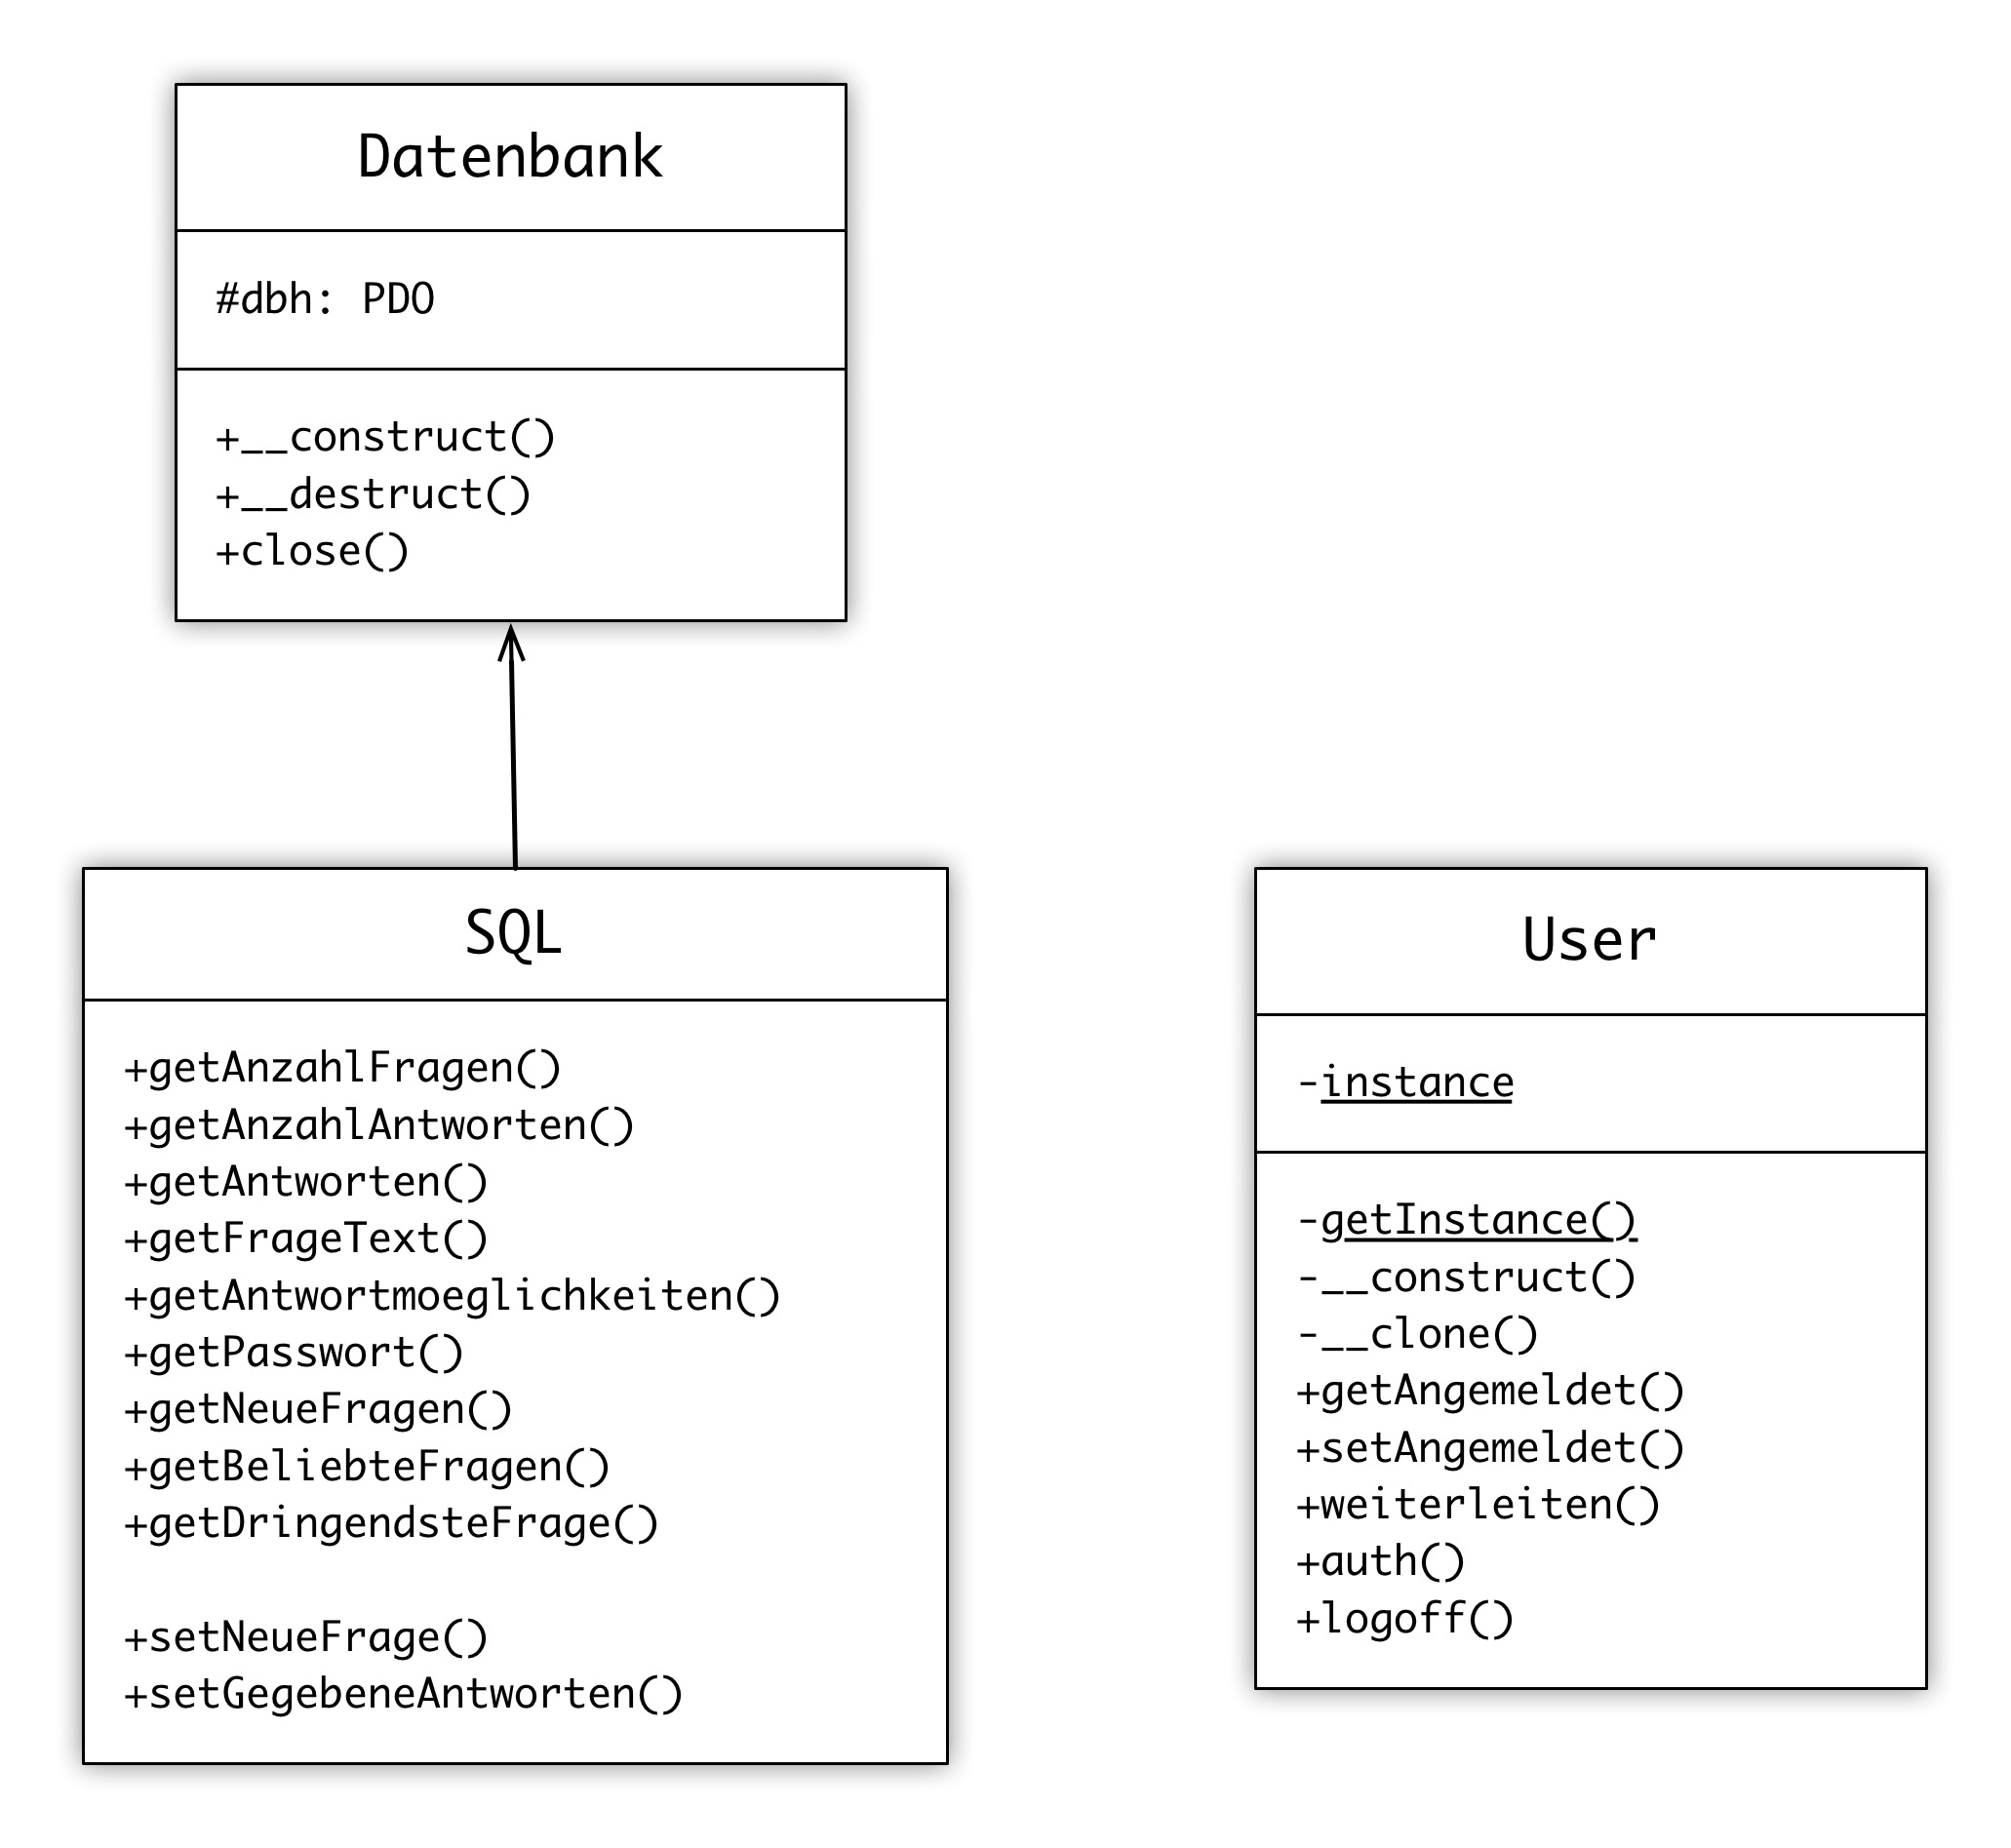
\includegraphics[width=\textwidth]{UML.jpg}
\caption{UML--Klassendiagramm}
\label{fig:uml}
\end{center}
\end{figure}

Die Implementation der Klassen ist im beigefügten Quelltext in den Dateien \code{.../class/Datenbank.php}, \code{.../class/SQL.php} und \code{.../class/User.php} zu betrachten. Auch die Klasse „User“ nutzt für den Datenbankzugriff die Klasse „SQL“. Dies geschieht allerdings nur innerhalb der Methode \code{auth()} über eine lokale Variable und ist daher im UML--Diagramm nicht zu erkennen.

\subsection{Klasse: Datenbank --- Low--Level Zugriff}

Die Klasse „Datenbank“ stellt die unterste Ebene des Datenzugriffs der Anwendung dar. Aufgrund der von PHP zur Verfügung gestellten PDO--Klasse greift jedoch auch diese Klasse nicht direkt auf die Datenbank  zu. Das PDO--Objekt ist als Attibut in der Klasse vorhanden. Die für den Zugriff notwendigen Angaben werden im Konstruktor aus der Konfigurationsdatei \code{.../includes/dbconf.ini} gelesen und anschließend wird die Verbindung zur Datenbank hergestellt. 

Die Datenbankverbindung bleibt so lange bestehen, wie die Instanz existiert. Ein Objekt mit geschlossener Datenbankverbindung würde die Notwendigkeit von zusätzlichen Fehlerprüfungen bzw. der erneuten Herstellung der Verbindung mit sich bringen. Um hierauf ausdrücklich hinzuweisen ist die Methode \code{close()} ohne Funktion definiert.
 
\subsection{Klasse: SQL --- High--Level Zugriff}

In der Klasse „SQL“ werden die SQL--Abfragen gekapselt. Der aufrufende PHP--Code benötigt keinerlei Wissen über die zu Grunde liegende Datenbank. Es müssen lediglich die Get-- und Set--Methoden eines Objektes vom Typ SQL aufgerufen werden. Innerhalb dieser Methoden werden dann die SQL--Abfragen mit Hilfe des geerbten PDO--Objekts vorbereitet und dann mit den geforderten Parametern aufgerufen. Die Ergebnisse werden dann als einzelner Wert oder als Objekt mit mehreren Werten bzw. Array zurückgegeben. Hierbei wird die jeweils geeignete Form gewählt.

Zum Speichern von neuen Fragen und Antwortmöglichkeiten bzw. von gegebenen Antworten werden diese an die entsprechenden Set--Methoden übergeben. Hierin werden die zum Abspeichern benötigten SQL-INSERTs in eine Transaktion verpackt. Somit ist auch bei gleichzeitigem Zugriff mehrerer Nutzer oder im Fehlerfall ein konsistenter Zustand des Datenbestandes gesichert.

Durch die Reduzierung der Aufrufe auf die passenden Get-- und Set--Methoden wird in der SQL-Klasse das Fassden-Entwurfsmuster realisiert. Der Aufrufende Code benötigt keinerlei Informationen über die Datenstruktur, die Datenbank oder Transaktionen. Änderungen an diesen technischen Details wirken sich lediglich auf die SQL--Klasse aus. So lange diese laut Spezifikation Werte entgegennimmt und zurückliefert, muss kein weiterer Programmcode geändert werden.

\subsubsection{Speichern von neuen Fragen und Antwortmöglichkeiten}
\label{sec:speichern}
In der Methode \code{setNeueFrage()} werden neue Fragen und die zugehörigen Antwortmöglichkeiten in der Datenbank abgespeichert. Hierzu werden die entsprechenden Texte in den Parametern \code{\$fragetext} und \code{\$antworten} übergeben werden. Bei letzterem handelt es sich um ein Array, da es pro Frage mehrere Antwortmöglichkeiten gibt.

Das Datenbankschema verlangt es, dass zu jeder Antwortmöglichkeit die ID der zugehörigen Frage gespeichert wird. Somit wird zunächst die Frage in die Datenbank eingefügt. Die automatisch generierte ID kann dann mit der PDO--Methode \code{lastInsertId()} ausgelesen werden. Anschließend werden die Antwortmöglichkeiten in einer \code{foreach}--Schleife in die Datenbank eingefügt.

Dieser Vorgang besteht somit aus vielen einzelnen Schritten. Fehlermöglichkeiten bestehen im PHP--Code selbst sowie beim Zugriff auf die Datenbank. An jeder Stelle sind Unterbrechungen durch weitere Instanzen der Anwendung möglich, was im schlimmsten Fall zu einer inkorrekten Frage--ID führen könnte. Es ist sicher zu stellen, dass entweder die gesamte Kombination von Frage mit allen zugehörigen Antwortmöglichkeiten gespeichert wird, oder das Speichern gar nicht statt findet und mit einer entsprechenden Fehlermeldung abbricht. Im Fehlerfall darf keine Frage ohne den kompletten Antwortsatz in der Datenbank sein. 

Daher wird der gesamte Vorgang in einer SQL--Transaktion eingebettet und im Fehlerfall werden schon getätigte Änderungen mit einem Rollback zurückgenommen. Somit ist Konsistenz der Datenbank zu jedem Zeitpunkt sichergestellt.

\subsection{Klasse: User --- Benutzerverwaltung}
\label{sec:user}
Die Benutzerverwaltung nutzt das Singleton Entwurfsmuster. Dieses wird durch die folgenden Maßnahmen implementiert: Die private Deklaration des Konstruktors sowie der \code{clone()} Methode wird die direkte Instanziierung der Klasse unterbunden. Eine Referenz auf die Instanz wird in der ebenfalls privaten statischen Variable \code{ \$instance } gespeichert und über die öffentliche Funktion \code{getInstance()} bekannt gemacht.

Die Funktion \code{auth()} erwartet als Parameter den Benutzernamen und das Passwort sowie optional eine URL zu der im Falle der erfolgreichen Authentifizierung umgeleitet werden soll. Der Datenbankzugriff erfolgt über eine lokale Instanz der Klasse SQL. Stimmen die Anmeldedetails mit den in der Datenbank gespeicherten überein werden in der von PHP zur Verfügung gestellten \code{\$\_SESSION}--Variable das Feld „angemeldet“ mit \code{TRUE} und das Feld „benutzer“ mit dem Benutzernamen gefüllt. Stimmen die Anmeldedaten nicht mit den gespeicherten Werten überein, so erhält das Feld „angemeldet“ den Wert \code{FALSE}.

Die Funktion \code{logoff()} meldet den momentan anfemeldeten Nutzer ab, in dem die Session-Variable zerstört und damit auch die Felder „angemeldet“ und „benutzer“ löscht.

Die Funktion \code{setAngemeldet()} ist eine private Hilfsmethode, mit der das Feld „angemeldet“ der \code{\$\_SESSION}--Variable gesetzt werden kann. Da sie aus der Methode \code{getInstance()} heraus aufgerufen wird, ist sie wie diese auch statisch deklariert.

Die Funktion \code{getAngemeldet()} dient zur Anfrage des Anmeldestatus. Sie wird immer dann aus der Anwendung heraus aufgerufen, wenn der Seitenaufbau für angemeldete Benutzer anders sein soll, wie für nicht angemeldete. Am auffällisten ist dies beim Aufruf der Seite zur Eingabe von neuen Fragen. Hier wird dem nicht angemeldeten Nutzer das Login--Formular angezeigt, wärend dem angemeldeten Nutzer die gewünschte Funktion direkt zur Verfügung steht.\\
Aber auch in Details können sich die Seiten unterscheiden: Die in der Seitenleiste angebotenen Links können schon entsprechend angepasst sein. Auf diese Weise werden dem Nutzer nur die Möglichkeiten gezeigt, die für ihn tatsächlich relevant sind. 
